%
\section{Architecture design}\label{sec:arch}
%
Our goal is to develop a convolutional neural network that is suitable for both image classification and instance retrieval.
%
%
%
In the current best practices, the architectures and training procedures used for class and instance recognition differ in a significant manner.
%

This section describes such technical differences, summarized in \cref{tab:diff_classif_instance}, together with our solutions to bridge them. 
This leads us to a unified architecture, shown in \cref{fig:3arch}, that we jointly train for both tasks in an end-to-end manner.


\begin{table}
\centering
\caption{\label{tab:diff_classif_instance}
Differences between classification and image retrieval:
Retrieval architectures incorporate a final pooling layer that is regionalized (RMAC) or magnifies activations (GeM). The triplet loss requires a batching strategy with pairs of matching images. %
%
}
\vspace{-7pt}
%
%
%
%
%
%
%
%
%
{\small
\begin{tabular}{@{}lc@{\hspace{5pt}}c@{}}
\toprule
                  & classification       & retrieval \\ 
\midrule 
spatial pooling   & avg. pooling         & RMAC~\cite{TOLIAS20143466} or GeM~\cite{radenovic2018fine} \\
loss              & cross-entropy        & triplet~\cite{Gordo2016DeepIR}  \\
batch sampling    & diverse              & similar images in batch  \\
whitening         & no                   & yes  \\
resolution        & low ($224^2$--$300^2$)           & high ($800$--$1$k$\times$scaled) \\
%
%
%
%
\bottomrule
\end{tabular}}

\vspace{-7pt}
\end{table}




\subsection{Spatial pooling operators\label{sec:p-pooling}}
%
%
%
%
%
%
%
%
%
%
%
This section considers the final, global spatial pooling layer.
%
Local pooling operators, usually max pooling, are found throughout the layers of most convolutional networks to achieve local invariance to small translations. 
By contrast, global spatial pooling converts a 3D tensor of activations produced by a convolutional trunk to a vector. 
%

\paragraph{Classification.}  
In early models such as LeNet-5~\cite{lecun1989backpropagation} or AlexNet~\cite{krizhevsky2012imagenet}, the final spatial pooling is just a linearization of the activation map.
It is therefore sensitive to the absolute location. 
Recent architectures such as ResNet and DenseNet employ average pooling, which is permutation invariant and hence offers a more global translation invariance. 
%
%
%

%
\begin{figure}
\centering
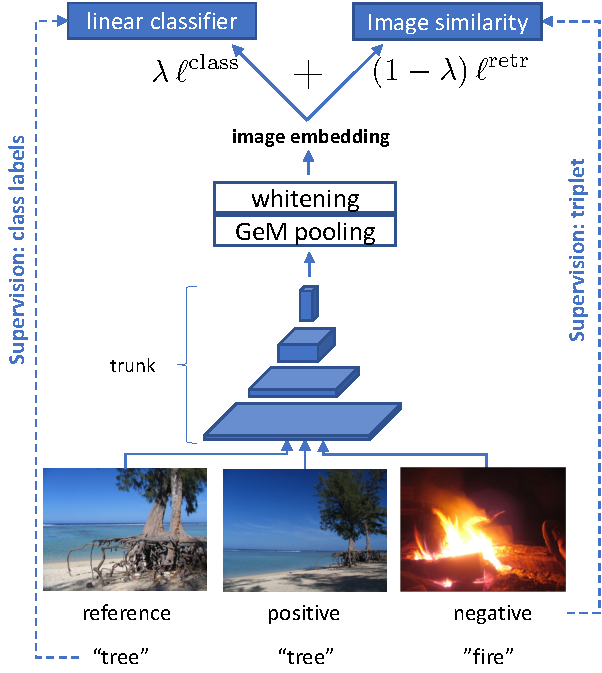
\includegraphics[width=0.9\linewidth]{figs/multigrain_rv}
\caption{\label{fig:3arch}
 Overview of our Multigrain architecture.} %
 \vspace{-10pt}
\end{figure}

\paragraph{Image retrieval}\hspace{-1em} requires more localized geometric information: particular objects or landmarks are visually more similar, but the task suffers more from clutter, and a given query image has no specific training data devoted to it. This is why the pooling operator tries to favor more locality. Next we discuss the generalized mean pooling operator. 

%
Let $\bx\in\mathbb{R}^{C\times W \times H}$ be the feature tensor computed by a convolutional neural network for a given image, where $C$ is the number of feature channels and $H$ and $W$ are the height and width of the map, respectively. 
We denote by $u\in\Omega=\{1,\dots,H\}\times\{1,\dots,W\}$ a ``pixel'' in the map, by $c$ the channel, and by $x_{cu}$ the corresponding tensor element: $\bx=[x_{cu}]_{c=1..C,u\in\Omega}$.
%
The generalized mean pooling (GeM) layer computes the generalized mean of each channel in a tensor.
Formally, the GeM embedding is given by
\begin{equation}\label{eq:gem}
 \be
 =
 \left[
 \Big(\frac{1}{|\Omega|}
 \sum_{u\in \Omega}x^p_{cu}
\Big)^\frac{1}{p}
 \right]_{c=1..C}
\end{equation}
where $p > 0$ is a parameter. Setting this exponent as $p>1$ increases the contrast of the pooled feature map and focuses on the salient features of the image~\cite{Bo2009EfficientMK,Boureau2010ATA,dollar2009integral}. 
%
GeM is a generalization of the average pooling commonly used in classification networks ($p=1$) and of spatial max-pooling layer ($p=\infty$). 
It is employed in the original R-MAC as an approximation of max pooling~\cite{dollar2009integral}, yet only recently~\cite{radenovic2018fine} it was shown to be competitive on its own with R-MAC for image retrieval.

%
To the best of our knowledge, this paper is the first to apply and evaluate GeM pooling in an image classification setting.
More importantly, we show later in this paper that \emph{adjusting the exponent is an effective way to change the input image resolution between train and test time} for all tasks, which explains why image retrieval has benefited from it considering that this task employs higher-resolution images. 

%
%
%
%
%
%
%
%
%
%
%
%
%
%
%
%
%

%
%

%

\subsection{Training objective\label{sec:losses}}

In order to combine the classification and retrieval tasks, we use a joint objective function composed of a classification loss and an instance retrieval loss. 
The two-branch architecture is illustrated in ~\cref{fig:3arch} and detailed next.

\paragraph{Classification loss.}

For classification, we adopt the standard cross-entropy loss.
Formally, let $\be_i\in\mathbb{R}^d$ be the embedding computed by the deep network for image $i$, $\bw_c \in \mathbb{R}^{d}$ the parameters of a linear classifier for class $c \in \{1,\dots,C\}$, and $y_i$ be the ground-truth class for that image.
Then
\begin{equation}\label{eq:crossent}
\lclass(\be_i,\bW,y_i)
=
- \langle \bw_{y_i}, \be_i \rangle
+ \log \sum_{c=1}^C
\exp \langle\bw_c, \be_i \rangle,
\end{equation}
where $\bW=[\bw_c]_{c=1..C}$.
We omit it for simplicity, but by adding a constant channel to the feature vector, the  bias of the classification layer is incorporated in its weight matrix. 


\paragraph{Retrieval loss.}

For image retrieval, the embeddings of two matching images (a positive pair) should have distances smaller than embeddings of non-matching images (a negative pair). 
%
This can be enforced in two ways. 
The contrastive loss~\cite{hadsell2006dimensionality} requires distances between positive pairs to be smaller than a threshold, and distances between negative pairs to be greater.
The triplet loss instead requires an image to be closer to a positive sibling than to a negative sibling~\cite{schroff2015facenet}, which is relative property of image triplets.
%
These losses requires adjusting multiple parameters, including how pairs and triplets are sampled. These parameters are sometimes hard to tune, especially for the triplet loss.

Wu~et~al.~\cite{wu2017sampling} proposed an effective method that addresses these difficulties.
Given a batch of images, they re-normalize their embeddings to the unit sphere, sample negative pairs as a function of the embedding similarity, and use those pairs in a margin loss, a variant of contrastive loss that shares some of the benefits of the triplet loss.

In more detail, given images $i,j\in\mathcal{B}$ in a batch with embeddings $\be_i,\be_j\in\mathbb{R}^d$, the margin loss is expressed as
\begin{equation}\label{eq:margin}
  \lret(\be_i, \be_j, \beta, y_{ij})
  = \max\{0, \alpha + y_{ij}(D(\be_i, \be_j) - \beta)\}
\end{equation}
where
$
%
    D(\be_i, \be_j) = \left\| \sfrac{\be_i}{\|\be_i\|} - \sfrac{\be_j}{\|\be_j\|}\right\|
$
%
is the Euclidean distance between the normalized embeddings, the label $y_{ij}$ is equal to 1 if the two images match and $-1$ otherwise, $\alpha > 0$ the margin (a constant hyper-parameter), and $\beta > 0$ is a parameter (learned during training together with the model parameters), controlling the volume of the embedding space occupied embedding vectors.
Due to the normalization, $D(\be_i, \be_j)$ is equivalent to a cosine similarity, which, up to whitening (\cref{sec:whiten}), is also used in retrieval.

%
%
%
%
%
%
%

Loss~\eqref{eq:margin} is computed on a subset of positive and negative pairs $(i,j)\in \mathcal{B}^2$ selected with the sampling~\cite{wu2017sampling} 
%
%
\begin{equation}
\begin{aligned}
\mathcal{P}_+(\mathcal{B})
&= \{ (i,j) \in \mathcal{B}^2: y_{ij} = 1\},
\\
\mathcal{P}_-(\mathcal{B})
&=
  \{ (i,j^*) : (i,j) \in \mathcal{P}_+(\mathcal{B}), 
  j^* \sim p(\cdot|i)
  \},
\\
\mathcal{P}(\mathcal{B})&=\mathcal{P}_+(\mathcal{B})\cup\mathcal{P}_-(\mathcal{B}),
\end{aligned}
\end{equation}
where the conditional probability of choosing a negative $j$ for image $i$ is 
$
 p(j|i) \propto \min\{\tau, q^{-1}(D(\be_i,\be_j))\} 
 \cdot \mathbf{1}_{\{y_{ij}=-1\}},
$
where $\tau > 0$ is a parameter and $q(z) \propto z^{d-2}(1 - z^2/4)^{\frac{d-3}{2}}$ is a PDF that depends on the embedding dimension $d$.

The use of distance weighted-sampling with margin loss is very suited to our joint training setting: this framework tolerates relatively small batch sizes ($|\mathcal{B}|\sim 80$ to $120$ instances) while requiring only a small amount of positives images (3 to 5) of each instance in the batch, without the need for elaborate parameter tuning or offline sampling.

\paragraph{Joint loss and architecture.}

The joint loss is a combination
of classification and retrieval loss weighted by a factor $\lambda \in [0, 1]$.
For a batch $\mathcal{B}$ of images, the joint loss writes as
\begin{equation}\label{eq:joint}
\frac{\lambda}{|\mathcal{B}|}\cdot\sum_{i\in\mathcal{B}}
\lclass(\be_i,\bw,y_i)
+
\frac{1-\lambda}{|\mathcal{P}(\mathcal{B})|}
\cdot\hspace{-1em}
\sum_{\raisebox{-3pt}{
$\scriptstyle(i,j)\in\mathcal{P}(\mathcal{B})$
}}
\hspace{-1em}
\lret(\be_i, \be_j, \beta, y_{ij}),
\end{equation}
\ie, losses are normalized by the number of items in the corresponding summations.


%
%
%

\subsection{Batching with repeated augmentation (RA)\label{sec:data-augmented-batches}}

%
%
Here, we propose to use only a training dataset for image classification, and train instance recognition via data augmentation.
%
The rationale is that data augmentation produces another image that contains the same object instance.
This approach does not require more annotation beyond the standard classification set.

%
%

%
%
%

We introduce a new sampling scheme for training with SGD and data augmentation, which we refer to as~\emph{repeated augmentations}.
In RA we form an image batch $\mathcal{B}$ by sampling $\left\lceil|\mathcal{B}|/m\right\rceil$ different images from the dataset, and transform them up to $m$ times by a set of data augmentations to fill the batch. 
Thus, the instance level ground-truth $y_{ij}=+1$ iff images $i$ and $j$ are two augmented versions of the same training image.
%
The key difference with the standard sampling scheme in SGD is that samples are not independent, as augmented versions of the same image are highly correlated. 
%
%
While this strategy reduces the performance if the batch size is small, for larger batch sizes RA outperforms the standard i.i.d.~scheme -- while using the same batch size and learning rate for both schemes.
This is different from the observation of~\cite{2019arXiv190109335H}, who also consider repeated samples in a batch, but simultaneously increase the size of the latter.

We conjecture that the benefit of correlated RA samples is to facilitate learning features that are invariant to the only difference between the repeated images --- the augmentations.
By comparison, with standard SGD sampling, two versions of the same image are seen only in different epochs. 
A study of an idealized problem illustrates this phenomenon in the supplementary material~\ref{sec:suppl-data-augmented-toy}.

\subsection{PCA whitening}\label{sec:whiten}

In order to transfer features learned via data augmentation to standard retrieval datasets, we apply a step of PCA whitening, in accordance
with previous works in image retrieval~\cite{Gordo2017EndtoEndLO,jegou2012negative}.
The Euclidean distance between transformed features is equivalent to the Mahalanobis distance between the input descriptors.
This is done after training the network, using an external dataset of unlabelled images. 


The effect of PCA whitening can be undone in the parameters of the classification layer, so that the whitened embeddings can be used for both classification and instance retrieval. In detail, let $\be$ be an image embedding vector and $\bw_c$ the weight vector for class $c$, such that $\langle\bw_c,\be\rangle$ are the outputs of the classifier as in~\cref{eq:crossent}.
The whitening operation $\Phi$ can be written as~\cite{Gordo2017EndtoEndLO}
$
    \Phi(\be) = S \left(\frac{\be}{\|\be\|} - \bm{\mu}\right)
$
given the whitening matrix $S$ and centering vector $\bm{\mu}$; hence
\begin{equation*}\label{eq:adapted_classifier}
    \langle\bw_c,\be\rangle = 
    \langle\bw_c,\Phi^{-1}(\Phi(\be))\rangle =
    \|\be\| \left( \langle\bw_c', \Phi(\be)\rangle + b_c' \right) 
\end{equation*}
where 
$
\bw_c' =  
S^{-1 \top} \bw_c
$
and
$
b_c' = \langle\bw_c, \mu \rangle
$
are the modified weight and bias for class $c$.
%
We observed that inducing decorrelation via a loss~\cite{Cogswell2016ReducingOI} is insufficient to ensure that features generalize well, which concurs with prior works~\cite{Gordo2017EndtoEndLO,radenovic2018fine}.


%

%
%
%

\subsection{Input sizes\label{sec:input-size}}

The standard practice in image classification is to resize and center-crop input images to a relatively low resolution, e.g.~$224\times 224$ pixels~\cite{krizhevsky2012imagenet}. 
%
The benefits are a smaller memory footprint, faster inference, and the possibility of batching the inputs if they are cropped to a common size. On the other hand, image retrieval is typically dependent on finer details in the images, as an instance can be seen under a variety of scales, and cover only a small amount of pixels.
The currently best-performing feature extractors for image retrieval therefore commonly use input sizes of $800$~\cite{Gordo2017EndtoEndLO} or $1024$~\cite{radenovic2018fine} pixels for the largest side, without cropping the image to a square.
This is impractical for end-to-end training of a joint classification and retrieval network.

Instead, we train our architecture at the standard $224\times 224$ resolution, and use larger input resolutions at test time only. 
This is possible due to a key advantage of our architecture:
a network trained with a pooling exponent $p$ and resolution $s$ can be evaluated at a larger resolution $s^*>s$ using a larger pooling exponent $p^*>p$, see our validation in \cref{sec:classif-results}. 

\label{sec:expanding-resolution}
\paragraph{Proxy task for cross-validation of $p^*$.} In order to select the exponent $p^*$, suitable for all tasks, we create a synthetic retrieval task {\bf \inaug} in between classification and retrieval. We sample $2,\!000$ images from the training set of ImageNet, $2$ per class, and create 5 augmented copies of each of them, using the ``full'' data augmentation described before. 

We evaluate the retrieval accuracy on \inaug in a fashion similar to UKBench~\cite{nister2006scalable}, with an accuracy ranging from 0 to 5 depending measuring how many of the first 5 augmentations are ranked in top 5 positions. 
We pick the best-performing $p^* \in \{1, 2,\ldots, 10\}$ on \inaug, 
which provides the following choices as a function of $\lambda$ and $s^*$:
%
\begin{equation*}
{\small
\begin{tabular}{c|lrrr}
\toprule
$\lambda$ & $s^*=$ & $224$ & $500$ & $800$ \\
\midrule
$1$   & $p^*=$ & $3$ & $4$ & $4$\\
$0.5$ & $p^*=$ & $3$ & $4$ & $5$\\
\bottomrule
\end{tabular}}
\end{equation*}

The optimal $p^*$ obtained on \inaug provides a trade-off between retrieval and classification. Experimentally, we observed that other choices are suitable for setting this parameter: %
fine-tuning the parameter $p^*$ alone using training inputs at a given resolution by back-propagation of the cross-entropy loss provides similar results and values of $p^*$.  


%
